\chapter{Introduction}
Systems in biology, medicine and many other areas are subject to their underlying and usually unknown dependency structures.
Clearly, learning these structures from available data could be invaluable, with the possibility of providing insight into a wide range of domain-specific problems.
This proves to be a difficult problem and especially so in high-dimensional settings, i.e. when there are many variables in relation to the available number of data samples.
This thesis focuses on the estimation of a subnetwork of such a dependency structure, namely the \gls{MB} of a few selected nodes of interest.
The  \gls{MB} is the set of nodes in a network that render a node of interest independent of the remaining network when being conditioned on. An example is shown in \autoref{fig:MB_shaded}.
\begin{figure}[H]
	\centering
	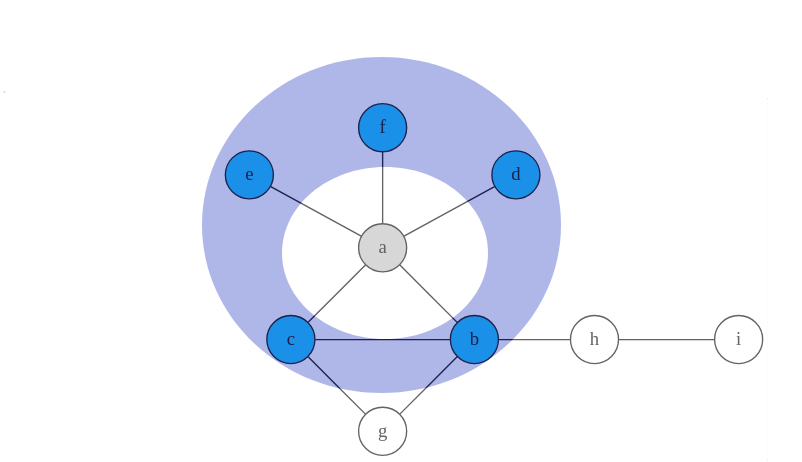
\includegraphics[width=0.5\textwidth]{MB_graph_shaded}
	\caption{The blue nodes form a \textit{blanket} around node 'a', rendering it conditionally independent of the remaining network.}
	
	\label{fig:MB_shaded}
\end{figure}

%When assuming that the data follows a multivariate Gaussian distribution, 
%In the setting of Gaussian Graphical Models (i.e. the assumption of multivariate normally distributed data) conditional independencies between variables are indicated by zero-entries of the inverse covariance matrix, which is also known as the precision matrix.
%With this in mind, the problem can be reformulated to the estimation of the precision matrix.
%In classical statistics this problem is traditionally referred to as "Covariance Selection".
In statistics the general problem of inferring the dependence structure of (assumed) Gaussian distributed data is classically known as \textit{Covariance Selection} \cite[]{price1972extension}, because the zero-pattern of the inverse covariance matrix encodes conditional independencies. 
Since dependence structures can be conveniently expressed in the form of a network graph (see \autoref{fig:cov_to_GMM}), the problem now tends to be referred to as the estimation of a \gls{GGM}.
\begin{figure}
	\hspace*{2cm}
	$\text{sign}(\matr{\Sigma^{-1}})=$
	$\Bigg($
	\begin{tabular}{cccc}
		\textbf{a} & \textbf{b} & \textbf{c} & \textbf{h}\\
		1&1&1&0\\
		1&1&1&-1\\
		1&1&1&0\\
		0&-1&0&1\\
		&&&
	\end{tabular}%
	$\Bigg)$
	\begin{tabular}{l}
		\\
		\textbf{{a}} \\
		\textbf{{b}} \\
		\textbf{{c}} \\
		\textbf{{h}} \\
		\\
	\end{tabular}
	$\Huge\Rightarrow$
	\makebox[0pt][l]{\raisebox{-10ex}{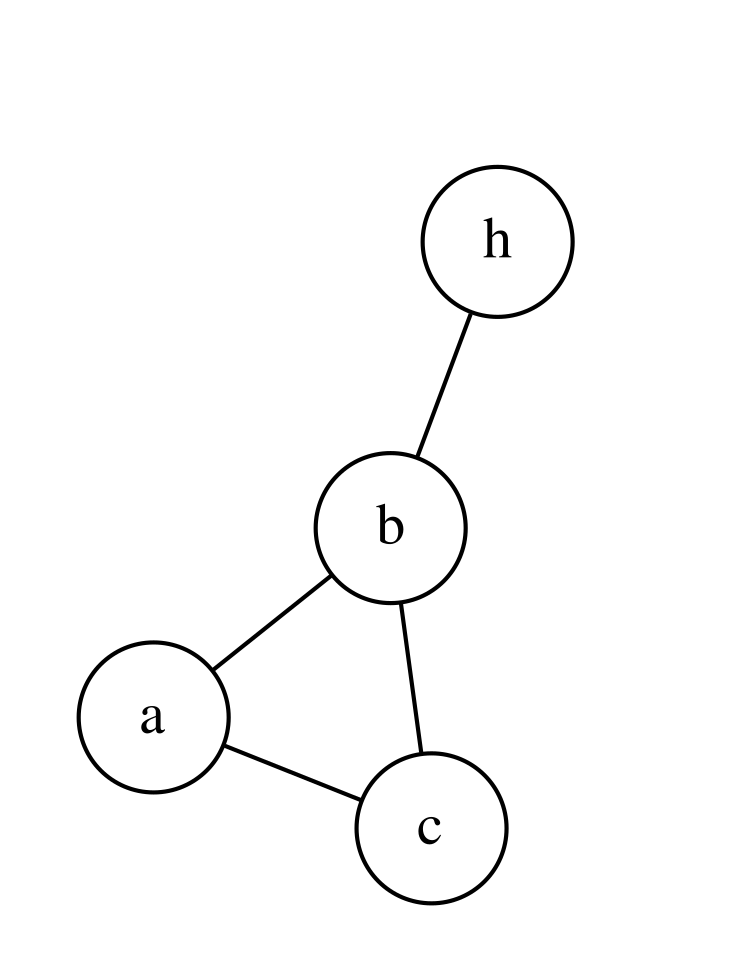
\includegraphics[width=0.2\textwidth]{MB_graph_small.png}}}%
\caption{Example for a dependency network encoded by the zero-pattern of the inverse covariance matrix.}
\label{fig:cov_to_GMM}
\end{figure}

Many popular approaches for estimating such \gls{GGM}s are based on enforcing sparsity in the network.
A sparse network is generally favorable for its interpretability, since large and densely connected graphs are difficult to analyze.
Prominent examples of sparse network estimation are the Graphical LASSO \cite[]{friedman_sparse_2008} and its Bayesian perspective \cite[]{wang_bayesian_2012}.
As with many alternative approaches, they infer the full network,
which is not always required for the problem at hand.
In many real-world problems there are often only a few variables of interest (e.g. clinical factors) which might interact with a great number of other variables (e.g. genetic markers).
The interactions between these few variables and the others are often the ones of highest interest.
In such cases inferring the whole network might be unnecessary and computationally expensive (especially for models that rely on simulation, such as \gls{MCMC} methods).
Consequently, it would be advantageous to limit estimation to the subnetwork of interest, and the \gls{BMB} estimation by \citet{kaufmann_bayesian_2015} offers such an approach.
By avoiding the inference of the whole network, the method allows for a more efficient estimation than related Bayesian methods (e.g. \citet{wang_bayesian_2012}) when the Markov Blanket of a few variables is of importance.
\citet{kaufmann_bayesian_2015} infer the whole posterior distribution.
However, in practice a point estimate is often desired, among others for the sake of interpretability and convenience.
While we could base this estimate on statistics such as the mean or median of the empirical posterior,
the most probable point, name the \gls{MAP}, would be more sensible in many cases.
However, estimating this mode from the empirical posterior distribution acquired by MCMC sampling poses some problems
in high dimensional settings.
The estimation would require some sort of binning or kernel density estimation,
which generally does not scale well for higher dimensions due to the 'curse of dimensionality' \citep{stone1980optimal, scott1991feasibility}.
Furthermore, if the mode is not surrounded by a lot of probability mass, the majority of the simulation time will be spent exploring regions of lower interest.
We address this issue by introducing \gls{SA} to the Bayesian Markov Blanket estimation, allowing for a direct and more robust estimation of the \gls{MAP}.
Because Simulated Annealing is seamlessly added on top of an already existing MCMC sampler,
small changes of the original model, such as the introduction of (hyper) priors, can be integrated into the MAP estimation.
Compared to the non-Bayesian approach, \gls{SA} also gives the advantage of having both the full posterior and a point estimate for the same model available, if it is desired.
Performance of the Annealing in comparison to the \gls{BMB} and the Graphical LASSO is evaluated on artificial data.
Furthermore, we investigate the modality of the posterior as well as the general behavior of the model
on both artificial and real data.

As already mentioned, learning dependencies inherent to the data can be very useful in medical domains.
In context of this thesis, we will focus on the area of HIV-1 treatment responses for individuals that
have been successfully treated for more than five years.
While current treatments are capable of suppressing the virus, it cannot be fully exterminated and dormant viral populations will multiply again after treatment stop. 
Furthermore, mutations of the virus might result in resistances that can affect current and future treatments.
We aim to find potential dependencies between resistance relevant mutations in latent viral populations and clinical factors that quantify the success of the treatments (e.g. the viral load and CD4 cell counts).
Additionally, dependencies between the clinical factors and the prior \& current treatment of the patients are of interest.
Discovering these dependencies might for example serve as a preliminary feature selection step for predicting the success of antiretroviral treatments for individual patients.
This serves as our motivation for estimating the Markov Blankets of the clinical factors.
The data used for this originates from the SystemsX.ch HIV-X project \citep{HIVX} and the Swiss HIV Cohort Study \citep{SHCS}.

The thesis is divided into 6 chapters.
After a short overview of existing related work, the general background required for the \gls{BMB} and \gls{SA} is given.
On top of a basic overview of used statistical tools, we elaborate on the need for enforcing sparsity in the process of network estimation. 
In the third chapter, the \gls{BMB} model itself as well as its extension are presented.
This is mostly limited to a theoretic overview.
Details regarding the implementation, as well as the setup for the artificially created data are discussed in the fourth chapter.
Subsequently, we present the results obtained from the application on both synthetic data and HIV.
Finally, a conclusion as well as an outlook for possible future work is given.

\section{Contributions}
With the general goals outlined, 
the contributions of this thesis can be summarized to the following points:
\begin{itemize}
	\item Introduction of Simulated Annealing to Bayesian Markov Blanket estimation \citep{kaufmann_bayesian_2015}
	\item Evaluation and Comparison of \gls{BMB}, \gls{SA} and the Graphical LASSO on artificial data
	\item Experimental study regarding the modality of the underlying model
	\item Analysis of potential dependencies in the SystemsX.ch HIV-X cohort data \citep{HIVX, SHCS} with Markov Blanket estimation
	
\end{itemize}